% https://tex.stackexchange.com/questions/79350/help-with-drawing-a-triangle-in-using-tikz
\documentclass[12pt]{standalone}
\usepackage{tikz}

\begin{document}
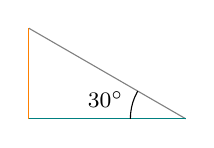
\begin{tikzpicture}
  \draw[gray] ++(150:2.3) -- (0,0);  %hypotenuse
  \draw[teal] ++(180:2) -- (0,0);    %adjacent
  \draw[orange] (-2,1.15) -- (-2,0); %opposite
  \path[clip] (0,0) -- (-2,0) -- (-2,1.15) -- cycle;
  \node[circle,draw,minimum size=40pt] at (0,0) (circ) {};
  \node[font=\footnotesize,left] at (circ.160) {$30^\circ$};
\end{tikzpicture}
\end{document}